\begin{equation*}
% a segment carries its coefficient; a sum is a branch, a product a series, and a route multiplies what it passes
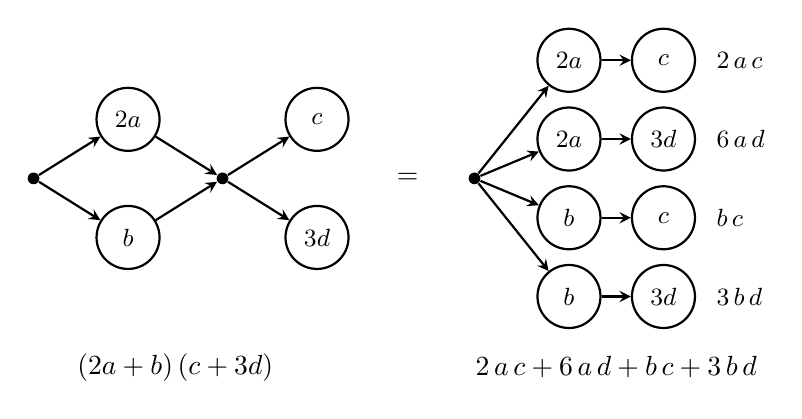
\begin{tikzpicture}[
  seg/.style={draw, circle, thick, minimum size=8mm, inner sep=0pt, font=\small},
  dot/.style={circle, fill, inner sep=1.5pt},
  hop/.style={thick, ->, >=stealth},
  note/.style={font=\small}
]
% a product of sums: (2a + b)(c + 3d), two branches in series
\node[dot] (s) at (0,0) {};
\node[seg] (A) at (1.2,0.75) {$2a$};
\node[seg] (B) at (1.2,-0.75) {$b$};
\node[dot] (m) at (2.4,0) {};
\node[seg] (C) at (3.6,0.75) {$c$};
\node[seg] (D) at (3.6,-0.75) {$3d$};
\draw[hop] (s) -- (A);
\draw[hop] (s) -- (B);
\draw[hop] (A) -- (m);
\draw[hop] (B) -- (m);
\draw[hop] (m) -- (C);
\draw[hop] (m) -- (D);
\node at (1.8,-2.4) {$(2a + b)\,(c + 3d)$};
\node at (4.75,0) {$=$};
% a sum of products: a branch of the four routes, each the product of the coefficients it passes
\node[dot] (S) at (5.6,0) {};
\foreach \i/\y/\first/\second/\term in {1/1.5/2a/c/2\,a\,c, 2/0.5/2a/3d/6\,a\,d, 3/-0.5/b/c/b\,c, 4/-1.5/b/3d/3\,b\,d} {
  \node[seg] (F\i) at (6.8,\y) {$\first$};
  \node[seg] (G\i) at (8.0,\y) {$\second$};
  \draw[hop] (S) -- (F\i);
  \draw[hop] (F\i) -- (G\i);
  \node[note, anchor=west] at (8.55,\y) {$\term$};
}
\node at (7.4,-2.4) {$2\,a\,c + 6\,a\,d + b\,c + 3\,b\,d$};
\end{tikzpicture}
\end{equation*}
